\section{Decision tree}

%%%%%%%%%%%%%%%%%%%%%%%%%%%%%%%
\subsection{Main idea}
The Decision Tree is a non-parametric supervised learning method used for classification and regression.
It predicts the response with a set of if-then-else decision rules derived from the data.
The deeper the tree, the more complex the decision rules and the closer the model fits the data.
The decision tree builds classification or regression models in the form of a tree structure. 
Each node in the tree further partions the feature space into smaller and smaller subsets 
while at the same time an associated decision tree is incrementally developed.
The final result is a tree with decision nodes and terminal nodes. 
A decision node has two or more branches.
Leaf node represents a classification or decision. 
The topmost decision node in a tree which corresponds to the best predictor is called the root node.
Decision trees can handle both categorical and numerical data.

An example of such a tree is depicted below in figure \ref{fig:decision_tree_example}.

\begin{figure}[H]
    \captionsetup{format=plain}
    \makebox[\textwidth]{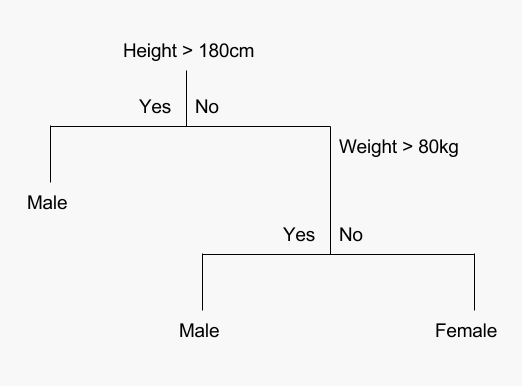
\includegraphics[width=100mm]{decision_tree_example.png}}
    \caption{Given a data set with two features height and weight, and gender as the target variable, 
             this example tree stratisfies the two-dimensional feature space into three distinct subset each 
             represented by the terminal nodes at the bottom.
             The stratification occurs at the two deciding nodes depending either on whether its height is above 180 cm 
             and or its weight  is above 80kg.
             }
    \label{fig:decision_tree_example}
\end{figure}

%%%%%%%%%%%%%%%%%%%%%%%%%%%%%%%
\subsection{Tree Building Process}
This chapter describes the CART algorithm for tree building as specified in \cite{breiman1984classification}.
The basic idea of tree growing is to choose a split among all the possible splits at each node
so that the resulting child nodes are the “purest”. In this algorithm, only univariate splits are
considered. That is, each split depends on the value of only one predictor variable. All
possible splits consist of possible splits of each predictor.

A tree is grown starting from the root node by repeatedly using the following steps on each
node (also called binary splitting)

\begin{itemize}
    \item[(i)] \textbf{Find best split \(s\) for each feature \(X_{m}\):}
    For each feature \(X_{m}\), there exist \(K-1\)-many potiential splits whereas \(K\) is the number of different values for the respective feature.
    Evaluate each value \(X_{m,i}\) at the current node \(t\) as a candidate split point (for \(x \in X_{m}\), if \(x \leq X_{m,i}=s\),
    then \(x\) goes to left child node \(t_{L}\) else to right child node \(t_{R}\)).
    The best split point is the one that maximize the splitting criterion \(\ \Delta i(s,t) \) the most when the node is split according to it.
    The different splitting criteria will be covered in the next chapter.
    \item[(ii)] \textbf{Find the node’s best split:} Among the best splits for each feature from Step (i) find the one \(s^{*}\), which maximizes the splitting criterion \(\Delta i(s,t)\).
    \item[(iii)] \textbf{Satisfy stopping criterion:} Split the node \(t\) using best node split \(s^{*}\) from Step (ii) and 
    repeat from Step (i) until stopping criterion is satisfied. 
\end{itemize}

%%%%%%%%%%%%%%%%%%%%%%%%%%%%%%%
\subsubsection{Splitting criteria}
Since we are only concerned with classification, \(Y\) is therefore categorical. The original CART algorithm uses Gini and Twoing as 
purity measures for the splitting criterion \cite{breiman1984classification}. However, implementations of the algorithm
such as Python's sklearn package \cite{scikit2011learn} also contain entropy and misclassification rate as measures of impurity.

For a given learning sample \( D = {(x_{1},y_{1}), (x_{2}, y_{2}), ... , (x_{N}, y_{N})} \) for a \(C\) class problem, let \(N_{c}\) be the number of instances \( \{x,y\}  \)
belonging to in class \(c\).

In node \(t\), let \(N(t)\) be the total number of instances with \( \{x,y\} \in t \) and \( N_{c}(t) \) the number of class \(c\)
cases in \(t\). The proportion of the class \(c\) instances in the sample \(L\) falling into \(t\) is  \( N_{c}(t) / N_{j} \).
For a given set of priors, \( \pi(c) \) is interpreted as the probability that an instance belongs to class \(c\).

At node \(t\), let the probabilities \(p(c,t)\) be estimated by 

\begin{equation}
    p(c,t) = \frac{ \pi(c)N_{c}(t) }{ N_{c} }.
\end{equation}

This represents the probability that an instance will both be  in class \(j\) and fall into node \(t\).
Therefore, the estimate for the probability that any instance falls into node \(t\) is defined by

\begin{equation}
    p(t) = \sum_{c \in C} p(c,t),
\end{equation}

The estimate \( p(t) \) for the probability that an instance belongs to class \(c\) given that it falls into node \(t\) is defined by

\begin{equation}
    p(c|t) = \frac{ p(c,t)}{ p(t) } = \frac{ p(c,t) }{ \sum_{c \in C} p(c,t) }.
\end{equation}

It holds that the conditional probability \(p(c|t)\) must satisfy

\begin{equation}
    \sum_{c \in C} p(c|t)  = 1
\end{equation}

Let \(i(t)\) be an impurity measure evaluated at note \(t\). Then, the decrease of impurity (i.e. the splitting criterion) is defined as

\begin{equation}
    \Delta i(s,t) = i(t) - p_{L} i(t_{L}) - p_{R} i(t_{R}),
\end{equation}

where \(p_{L}\) and \(p_{R}\) are probabilities of sending a case to the left child node \(t_{L}\) and to the
right child node \(t_{R}\) respectively. 
They are estimated as \( p_{L} = p(t_{L}) / p(t) \) and \( p_{R} = p(t_{R}) / p(t) \).

As already stated abobe, the goal is to maximize \(\Delta i(s,t)\).
In the following, different measures for impurity will be presented.

\textbf{Gini Measure}

The Gini impurity measure is defined as 


\begin{equation}
    i(t) = \sum_{c \in C} p(c|t) (1 - p(c|t)) = 1 - \sum_{c \in C} p_{c}^{2}
\end{equation}

The intuition behind this measure is to assign nodes for which its probabilities are more skewed towards a particular group a higher value.
Conversely, if a node has more balanced distribution, then \(i(t)\) will turn out to be lower.
For example, in the case of \( |C|=2 \), \(i(t)\) will be maximized by \( p(c|t) = 0.5 \) for \( c \in C \).


\textbf{Information Entropy}

The Entropy measure from information theory is defined as

\begin{equation}
    i(t) = \sum_{c \in C} p(c|t) log(p(c|t))
\end{equation}

which measures the average rate at which information is produced by a stochastic source of data .
Thus, it can also be used for measuring impurity.

\newpage

\textbf{Rate of Misclassification}

The rate of misclassification is defined as 

\begin{equation}
    i(t) = 1 - \max_{c \in C} p(c|t) .
\end{equation}

which measure the proportion of instances node \(t\) not belonging to the dominant group in \(t\).


%%%%%%%%%%%%%%%%%%%%%%%%%%%%%%%%%%%%%
\subsubsection{Bias-variance trade-off}
To measure the fit of a model to data, the generalization error is a widely used concept from \cite{breiman2001random}. 
Principally, we use generalization error to compare methods and adjust parameters to improve methods. 
Under certain assumptions, we can decompose the generalization error into three main components; the Bayes Error, 
the squared bias ($bias^2$) and the variance. 
We will explain the mathematical aspects of the generalization error in the following chapters. 
For now, we only need to mention the Bayes Error is irreducible and independent of the classifier, 
and there is a trade-off between $bias^2$ and variance. Since decision trees suffer from high variance and 
decreasing variance causes $bias^2$ to increase, we need methods to bypass this trade-off. 
Methods including Bagging, Boosting and Random Forest exploits mathematical properties to decrease variance 
without increasing $bias^2$. We will explain bagging briefly, exhibit mathematical dynamics of Random Forest and 
use Boosting in the application section.


\subsection{Bagging}
It is easy to guess that decision trees belong to methods which are sensitive to the specific data on which they are trained. It means that when we change training data 
we can get much different resulting decision trees and as a result of that also predictions are different. 
Bagging was created for these kind of methods which has high variance, like classification and regression trees.
Bagging or in other words Bootstrap Aggregation is a procedure that can be used for reducing the variance.
As a first step in bagging procedure we do bootstrapping, so we have to create many random subsample datasets with replacement
and then we use these datasets as training data for our model for example in our case decision tree. As a result we have the same number
of decision trees as the number of created datasets. Last step is to use new dataset to predict the result from each model and finally average the result 
over all unit results. After introducing bagged decision trees, another improvement to this method was created. Method which is an improvement over bagged decision trees 
is commonly known as the Random Forest which is the topic of our next section of paper.
